\chapter{Architectural description}

\section{Architecure}

\subsection{Architectural viewport selection}
The “4+1 view model” by Philippe Kruchten suggest four different view, logical, process, development and physical. In the case of XOXOMail we are going to use the logical, process and development view. The rationale behind removing the physical view is that XOXOMail will run on a single physical device and only utilize one process, a security view, describing the layers of security will be added instead.

\subsection{Logical view (Object oriented deomposition)}
“The logical architecture primarily supports the functional requirements --- what the system should provide in terms of services to its users. The system is decomposed into a set of key abstractions, taken from the problem domain, in the form of objects or object classes” \# A common way to represent this is view is with a class diagram that shows a set of classes and their relationships.
See figure \ref{fig:logicalview} at page \pageref{fig:logicalview}.

\begin{figure}
	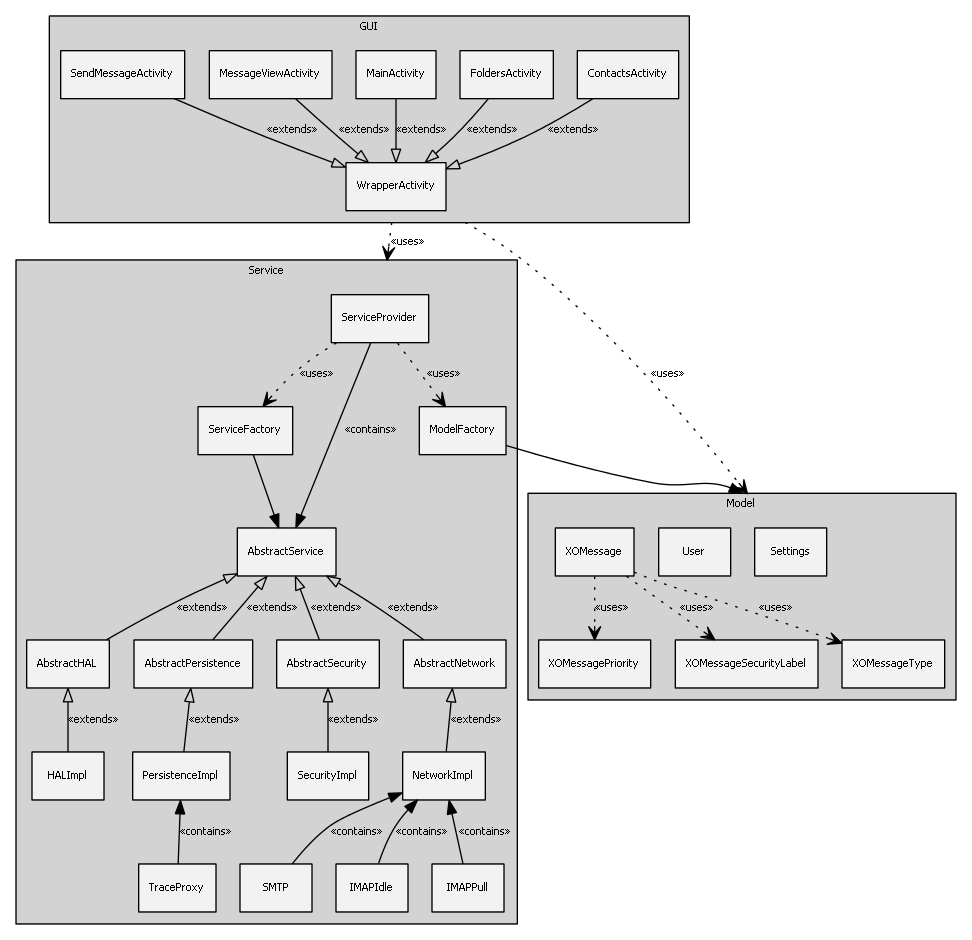
\includegraphics[width=\textwidth]{logicalview.png}
	\caption{The logical view of the architecture}
	\label{fig:logicalview}
\end{figure}

\subsection{Development view (Subsystem decomposition)}
The development view is a step up from the logical view and focuses on software modules instead of classes. These subsystems/modules are organized in a hierarchy of layers where each layer provides a well-defined interface to layers above. “The complete development architecture can only be described when all the elements of the software have been identified. It is, however, possible to list the rules that govern the development architecture: partitioning, grouping, visibility.“
See figure \ref{fig:developmentview} at page \pageref{fig:developmentview}.

\begin{figure}
	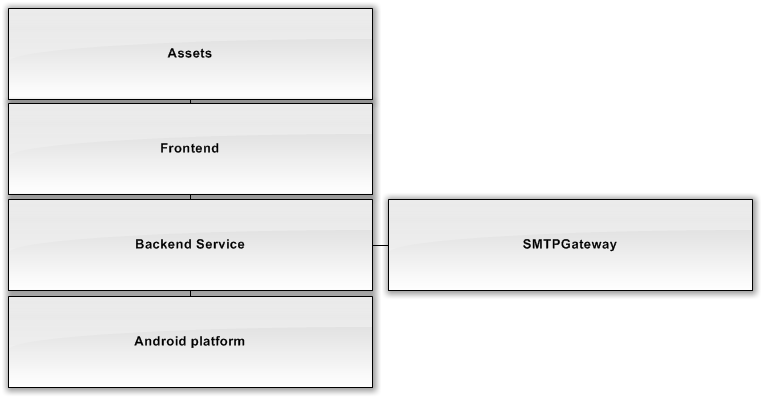
\includegraphics[width=\textwidth]{developmentview.png}
	\caption{Development View}
	\label{fig:developmentview}
\end{figure}

\subsection{Process View}
The process view is concerned with how different tasks bind together to form one executable unit. More specifically, the communication between threads/processes and on which thread/process is a task executed. We will differentiate between major and minor tasks, where major tasks are architectural elements open through a public interface, and minor tasks being tasks introduced in order to implement some functionality in one class or module.
See figure \ref{fig:processview} at page \pageref{fig:processview}.

\begin{figure}
	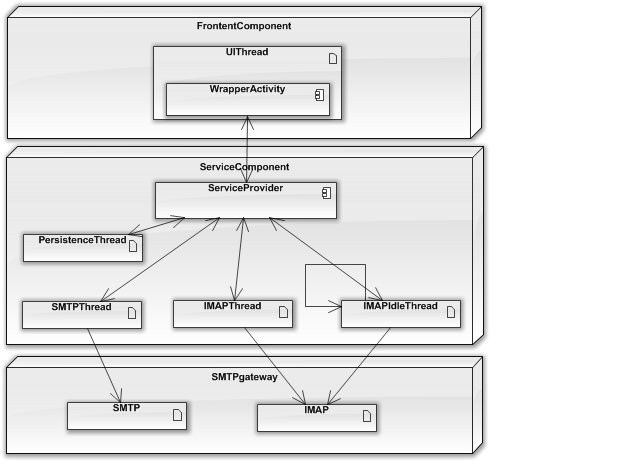
\includegraphics[width=\textwidth]{processview.png}
	\caption{Process view}
	\label{fig:processview}
\end{figure}

\subsection{Security View}
The security view is concerned with how the system as a whole is secured. This involves intercommunication, storage and communication with external sources. The view is not however concerned about implementation, just the layers of security.
See figure \ref{fig:securityview} at page \pageref{fig:securityview}.

\begin{figure}
	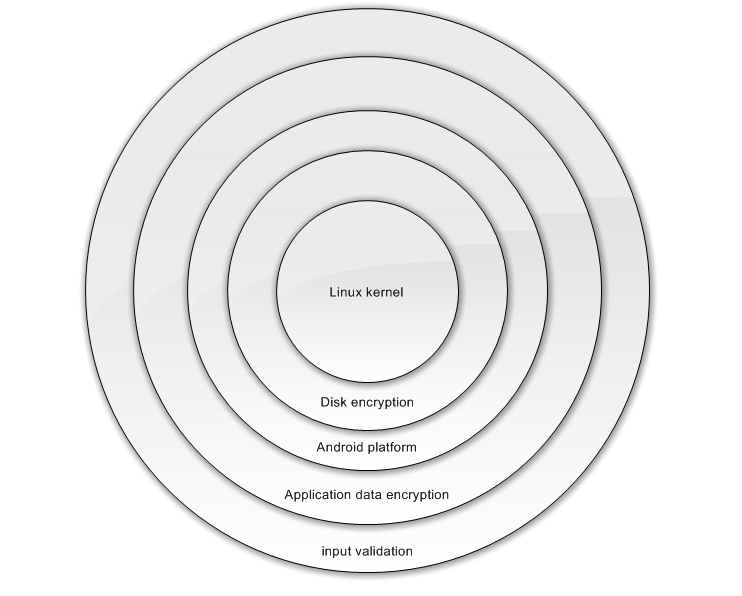
\includegraphics[width=\textwidth]{securityview.png}
	\caption{Security view}
	\label{fig:securityview}
\end{figure}

\textbf{The Linux kernel} provides us with a user-based permissions model and process isolation, which ensures that another process cannot access the memory of XOXOMail during runtime.
\newline
\newline
\textbf{Disk encryption}, is feature provided by the android platform, which encrypts the whole android device using AES with CBC and ESSIV:SHA256.
\newline
\newline
\textbf{Android platform}, most of the security provided by the android platform is provided by the linux kernel, but not necessary used in normal conditions. The application sandbox is one of these things. And since the sandboxing operation is located at kernel level, it is hard to break out of. 
\newline
\newline
\textbf{Application data encryption}, is a response to the possibility of rooted devices. Normally an android application will not run with root access on the device, this however is not the case on rooted devices. In which case the application and user will have full access to all applications and all application data. By adding our own encryption layer with the key stored off-device we can ensure data security even with root access to the phone. The encryption we opted for is an AES based encryption with a user-password derived key by PBKDF2-HMAC-SHA1.
Regarding communication with external resources as a mail-server, it will be done over a secure communication channel providing SSL or TLS. 
\newline
\newline
\textbf{Input validation}, is always necessary in order to provide a secure service. All input to the XOXOMail application should be validated, this is includes received mail, user-input etc. For mail validation we are going to use S/MIME signing and verification provided by bouncycastle. 



\subsection{GUI}
\begin{figure}
	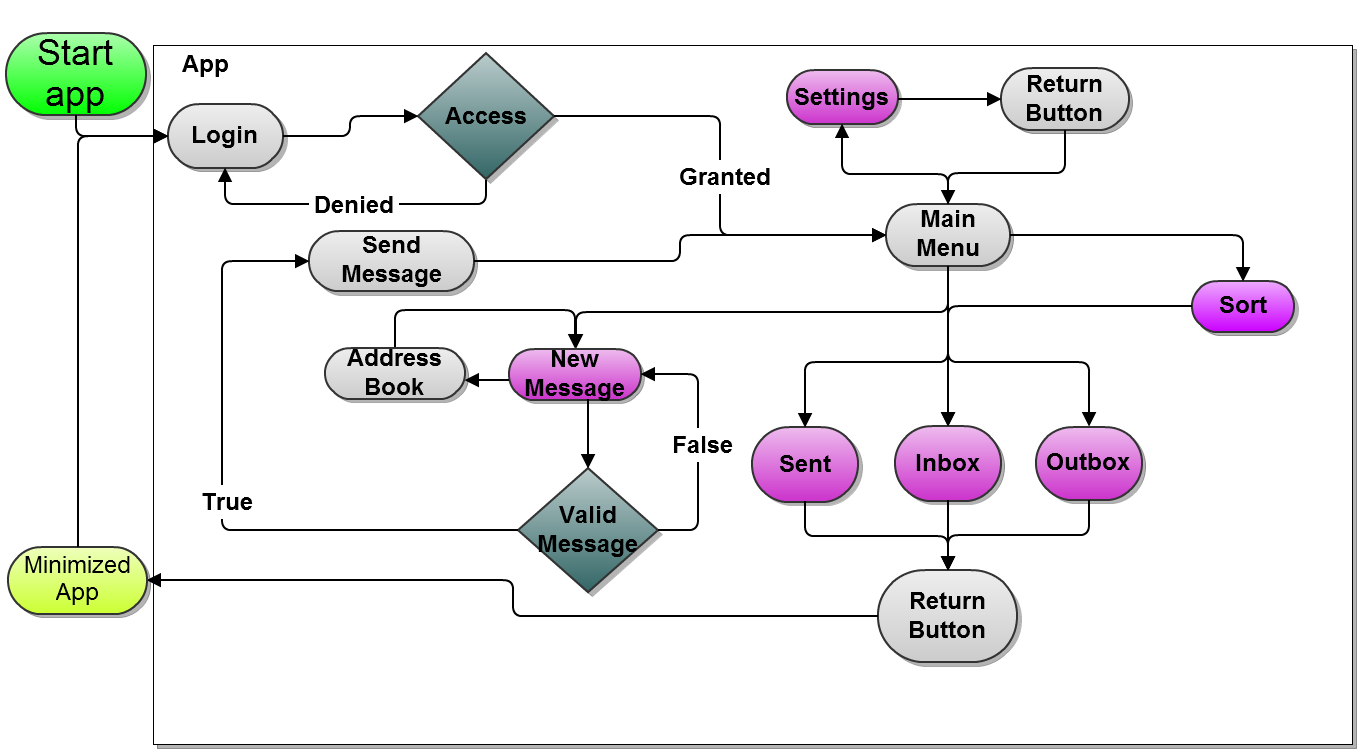
\includegraphics[width=\textwidth]{Android_GUI_flow_chart_2}
	\caption{The logical view of the GUI architecture}
	\label{fig:logicalGUIview}
\end{figure}